%%%%%%%%%%%%%%%%%%%%%%%%%%%%%%%%%%%%%%%%%
% Masters/Doctoral Thesis 
% LaTeX Template
% Version 2.5 (27/8/17)
%
% This template was downloaded from:
% http://www.LaTeXTemplates.com
%
% Version 2.x major modifications by:
% Vel (vel@latextemplates.com)
%
% This template is based on a template by:
% Steve Gunn (http://users.ecs.soton.ac.uk/srg/softwaretools/document/templates/)
% Sunil Patel (http://www.sunilpatel.co.uk/thesis-template/)
%
% Template license:
% CC BY-NC-SA 3.0 (http://creativecommons.org/licenses/by-nc-sa/3.0/)
%
%%%%%%%%%%%%%%%%%%%%%%%%%%%%%%%%%%%%%%%%%

%----------------------------------------------------------------------------------------
%   PACKAGES AND OTHER DOCUMENT CONFIGURATIONS
%----------------------------------------------------------------------------------------

\documentclass[
11pt, % The default document font size, options: 10pt, 11pt, 12pt
%oneside, % Two side (alternating margins) for binding by default, uncomment to switch to one side
english, % ngerman for German
singlespacing, % Single line spacing, alternatives: onehalfspacing or doublespacing
%draft, % Uncomment to enable draft mode (no pictures, no links, overfull hboxes indicated)
%nolistspacing, % If the document is onehalfspacing or doublespacing, uncomment this to set spacing in lists to single
%liststotoc, % Uncomment to add the list of figures/tables/etc to the table of contents
%toctotoc, % Uncomment to add the main table of contents to the table of contents
%parskip, % Uncomment to add space between paragraphs
%nohyperref, % Uncomment to not load the hyperref package
headsepline, % Uncomment to get a line under the header
%chapterinoneline, % Uncomment to place the chapter title next to the number on one line
%consistentlayout, % Uncomment to change the layout of the declaration, abstract and acknowledgements pages to match the default layout
]{MastersDoctoralThesis} % The class file specifying the document structure

\usepackage[utf8]{inputenc} % Required for inputting international characters
\usepackage[T1]{fontenc} % Output font encoding for international characters

\usepackage{mathpazo} % Use the Palatino font by default

\usepackage[backend=bibtex,style=authoryear,natbib=true]{biblatex} % Use the bibtex backend with the authoryear citation style (which resembles APA)

\addbibresource{retinopathy.bib} % The filename of the bibliography

\usepackage[autostyle=true]{csquotes} % Required to generate language-dependent quotes in the bibliography


% My usepackages
%%% Packages %%%
\usepackage{graphicx}
\usepackage{epsfig}
%\usepackage{subfigure}
\usepackage{caption} % subfigures
\usepackage[utf8]{inputenc}

% Needed for some foreign characters
\usepackage[T1]{fontenc}

\usepackage{smartdiagram}
%\newcommand{\degree}{\ensuremath{^{\circ}}\xspace} % adds degree sign 
% forced line break inside a tabular cell
\newcommand{\specialcell}[2][c]{%
	\begin{tabular}[#1]{@{}c@{}}#2\end{tabular}}

% use it for example as \specialcell[t]{Foo\\bar} or \specialcell{Foo\\bar}
%%%%%%%%%%%%%%%
\usepackage{rotating} % rotate elements in LaTeX
\usepackage{booktabs} % table formatting
\usepackage{wrapfig} % wrapping text around figures
\usepackage{caption} % subfigures
\usepackage{subcaption} % subfigures
\usepackage{makecell} % \thead in tables
\usepackage{amsmath}
\usepackage{amsfonts}
\usepackage{amssymb} % mathematical symbols
\usepackage{bm} % bold mode \bm
\usepackage{multicol}
\usepackage{xcolor}
\usepackage{amsmath}
%\usepackage{subfigure}
\usepackage{amsfonts}
\usepackage{amsthm}
\usepackage{multirow}
\usepackage{colortbl}
\usepackage{booktabs}
% This allows us to cite chapters by name, which was useful for making the
% acknowledgements page
\usepackage{nameref}
% Make sure there is a space between the subsection number and subsection title
% in the table of contents.
% If we do not do this we end up with 2 digit subsection numbers colliding with
% the title.
% See https://tex.stackexchange.com/questions/7853/toc-text-numbers-alignment/7856#7856?newreg=d2632892dd0345f388619f12fa794b11
\usepackage[tocindentauto]{tocstyle}
\usetocstyle{standard}

\usepackage{bm}


\usepackage{float}
\newcommand{\boldindex}[1]{\textbf{\hyperpage{#1}}}
\usepackage{makeidx}\makeindex
% Make bibliography and index appear in table of contents
\usepackage[nottoc]{tocbibind}
% Using the caption package allows us to support captions that contain "itemize" environments.
% The font=small option makes the text of captions smaller than the main text.
\usepackage[font=small]{caption}


\usepackage[chapter]{algorithm}
\usepackage{algorithmic}
% Include chapter number in algorithm number
\renewcommand{\thealgorithm}{\arabic{chapter}.\arabic{algorithm}}


\theoremstyle{definition}
\newtheorem{example}{Example}[section]

\newtheorem{theorem}{Theorem}%[section]
\newtheorem{corollary}{Corollary}[theorem]
\newtheorem{lemma}[theorem]{Lemma}
\theoremstyle{definition} % definition
\newtheorem{definition}{Definition}%[section]
\newtheorem{proposition}{Proposition}%[section]


\theoremstyle{remark}
\newtheorem*{remark}{Remark}

\newcommand{\me}{\mathrm{e}} % exponential e

% Define the P table cell environment
% It is the same as p, but centers the text horizontally
\usepackage{array}
\newcolumntype{P}[1]{>{\centering\arraybackslash}p{#1}}

% Rebuild the book document class's headers from scratch, but with different font size
% (this is for MIT Press style)
% Source: http://texblog.org/2012/10/09/changing-the-font-size-in-fancyhdr/
\newcommand{\changefont}{% 1st arg to fontsize is font size. 2nd arg is the baseline skip. both in points.
	\fontsize{9}{11}\selectfont
}

\input{math_commands.tex}

% End my usepackages


%----------------------------------------------------------------------------------------
%   MARGIN SETTINGS
%----------------------------------------------------------------------------------------

\geometry{
    paper=a4paper, % Change to letterpaper for US letter
    inner=2.5cm, % Inner margin
    outer=3.8cm, % Outer margin
    bindingoffset=.5cm, % Binding offset
    top=1.5cm, % Top margin
    bottom=1.5cm, % Bottom margin
    %showframe, % Uncomment to show how the type block is set on the page
}

%----------------------------------------------------------------------------------------
%   THESIS INFORMATION
%----------------------------------------------------------------------------------------

\thesistitle{Diabetic Retinopathy Classification and Interpretation using Deep Learning Techniques} % Your thesis title, this is used in the title and abstract, print it elsewhere with \ttitle
\supervisor{Dr. A\"ida \textsc{Valls} and \\Dr. Dom\`enec \textsc{Puig}} % Your supervisor's name, this is used in the title page, print it elsewhere with \supname
\examiner{} % Your examiner's name, this is not currently used anywhere in the template, print it elsewhere with \examname
\degree{Doctor of Philosophy} % Your degree name, this is used in the title page and abstract, print it elsewhere with \degreename
\author{Jordi \textsc{de la Torre}} % Your name, this is used in the title page and abstract, print it elsewhere with \authorname
\addresses{} % Your address, this is not currently used anywhere in the template, print it elsewhere with \addressname

\subject{Machine Learning and Artificial Intelligence} % Your subject area, this is not currently used anywhere in the template, print it elsewhere with \subjectname
\keywords{} % Keywords for your thesis, this is not currently used anywhere in the template, print it elsewhere with \keywordnames
\university{\href{http://www.urv.cat}{Universitat Rovira i Virgili}} % Your university's name and URL, this is used in the title page and abstract, print it elsewhere with \univname
\department{\href{http://deim.urv.cat}{Department d'Enginyeria Inform\`atica i Matem\`atiques de la Seguretat}} % Your department's name and URL, this is used in the title page and abstract, print it elsewhere with \deptname
\group{\href{http://deim.urv.cat/~itaka/}{ITAKA and RiVI Groups}} % Your research group's name and URL, this is used in the title page, print it elsewhere with \groupname
\faculty{\href{http://www.etse.urv.cat}{Escola T\`ecnica Superior d'Enginyeria}} % Your faculty's name and URL, this is used in the title page and abstract, print it elsewhere with \facname

\AtBeginDocument{
\hypersetup{pdftitle=\ttitle} % Set the PDF's title to your title
\hypersetup{pdfauthor=\authorname} % Set the PDF's author to your name
\hypersetup{pdfkeywords=\keywordnames} % Set the PDF's keywords to your keywords
}

% Allow align environments to cross page boundaries.
% If we do not do this, we get weird gaps of several inches of white space
% before or after some long align environments.
\allowdisplaybreaks

\begin{document}

%%% REQUIRED BY NOTATION CHAPTER
\setlength{\parskip}{0.25 \baselineskip}
\newlength{\figwidth}
\setlength{\figwidth}{26pc}
% Spacing between notation sections
\newlength{\notationgap}
\setlength{\notationgap}{1pc}
%%% REQUIRED BY NOTATION CHAPTER

\frontmatter % Use roman page numbering style (i, ii, iii, iv...) for the pre-content pages

\pagestyle{plain} % Default to the plain heading style until the thesis style is called for the body content

%----------------------------------------------------------------------------------------
%   TITLE PAGE
%----------------------------------------------------------------------------------------

\begin{titlepage}
\begin{center}

\vspace*{.06\textheight}
{\scshape\LARGE \univname\par}\vspace{1.5cm} % University name
\textsc{\Large Doctoral Thesis}\\[0.5cm] % Thesis type

\HRule \\[0.4cm] % Horizontal line
{\huge \bfseries \ttitle\par}\vspace{0.4cm} % Thesis title
\HRule \\[1.5cm] % Horizontal line
 
\begin{minipage}[t]{0.4\textwidth}
\begin{flushleft} \large
\emph{Author:}\\
\href{http://jorditg.github.io}{\authorname} % Author name - remove the \href bracket to remove the link
\end{flushleft}
\end{minipage}
\begin{minipage}[t]{0.4\textwidth}
\begin{flushright} \large
\emph{Supervisors:} \\
%\href{http://www.jamessmith.com}
{\supname} % Supervisor name - remove the \href bracket to remove the link  
\end{flushright}
\end{minipage}\\[3cm]
 
\vfill

\large \textit{A thesis submitted in fulfillment of the requirements\\ for the degree of \degreename}\\[0.3cm] % University requirement text
\textit{in the}\\[0.4cm]
\groupname\\\deptname\\[2cm] % Research group name and department name
 
\vfill

{\large \today}\\[4cm] % Date
%\includegraphics{Logo} % University/department logo - uncomment to place it
 
\vfill
\end{center}
\end{titlepage}

%----------------------------------------------------------------------------------------
%   DECLARATION PAGE
%----------------------------------------------------------------------------------------

\begin{declaration}
\addchaptertocentry{\authorshipname} % Add the declaration to the table of contents
\noindent I, \authorname, declare that this thesis titled, \enquote{\ttitle} and the work presented in it are my own. I confirm that:

\begin{itemize} 
\item This work was done wholly or mainly while in candidature for a research degree at this University.
\item Where any part of this thesis has previously been submitted for a degree or any other qualification at this University or any other institution, this has been clearly stated.
\item Where I have consulted the published work of others, this is always clearly attributed.
\item Where I have quoted from the work of others, the source is always given. With the exception of such quotations, this thesis is entirely my own work.
\item I have acknowledged all main sources of help.
\item Where the thesis is based on work done by myself jointly with others, I have made clear exactly what was done by others and what I have contributed myself.\\
\end{itemize}
 
\noindent Signed:\\
\rule[0.5em]{25em}{0.5pt} % This prints a line for the signature
 
\noindent Date:\\
\rule[0.5em]{25em}{0.5pt} % This prints a line to write the date
\end{declaration}

\cleardoublepage

%----------------------------------------------------------------------------------------
%   QUOTATION PAGE
%----------------------------------------------------------------------------------------

\vspace*{0.2\textheight}

\noindent\enquote{\itshape Study hard what interests you the most in the most undisciplined, irreverent and original manner possible.}\bigbreak

\hfill Richard Feynman

%----------------------------------------------------------------------------------------
%   ABSTRACT PAGE
%----------------------------------------------------------------------------------------

\begin{abstract}
\addchaptertocentry{\abstractname} % Add the abstract to the table of contents

Diabetic Retinopathy (DR) is a leading disabling chronic disease  and  one of the main causes of blindness and visual impairment in developed countries for diabetic patients. Studies reported that 90\% of the cases can be prevented through early detection and treatment. Eye screening through retinal images is used by physicians to detect the lesions related with this disease. Due to the increasing number of diabetic people, the amount of images to be manually analyzed is becoming unaffordable. Moreover, training new personnel for this type of image-based diagnosis is long, because it requires to acquire expertise by daily practice. 

In this thesis we explore different novel methods for the automatic classification of retina images.For this purpose, we explore methods based in automatic feature extraction and classification based on deep neural networks. Furthermore, as the conclusions of these models are difficult to analyze, we design a new method for the interpretation of the results reported by such models. The designed model is designed in a modular way in order to generalize its possible application to other networks and classification domains. We experimentally demonstrate that our interpretation model is able to detect retina lesions in the image solely from the classification information.

Furthermore, we identify the independent elements causing the disease from the feature extracted information of the designed models. With such information we are able to identify three visual independent causes for the disease. Using the designed interpretation method we are also able to identify on the image such independent components.

Finally, we applied our trained model for classifying retina images of a different population, concretely from the Hospital de Reus. We study the possible presence of co-variate shift between both populations and present the results obtained from such a new population. Results show that there is no significant co-variate shift between both populations and that the model can be directly used for prediction.
\end{abstract}

%----------------------------------------------------------------------------------------
%   ACKNOWLEDGEMENTS
%----------------------------------------------------------------------------------------

\begin{acknowledgements}
\addchaptertocentry{\acknowledgementname} % Add the acknowledgements to the table of contents

This work is supported by the URV grant 2015PFR-URV-B2-60 and the Spanish research projects PI15/01150 and PI12/01535 (Instituto Salud Carlos III). 

I would like to express my gratitude to my supervisors Dra A\"ida Valls and Dr Dom\`enec Puig for their useful guidance, insightful comments, and considerable encouragement to complete this thesis. 
\end{acknowledgements}

%----------------------------------------------------------------------------------------
%   LIST OF CONTENTS/FIGURES/TABLES PAGES
%----------------------------------------------------------------------------------------

\tableofcontents % Prints the main table of contents

\listoffigures % Prints the list of figures

\listoftables % Prints the list of tables

%----------------------------------------------------------------------------------------
%   ABBREVIATIONS
%----------------------------------------------------------------------------------------

\begin{abbreviations}{ll} % Include a list of abbreviations (a table of two columns)

\textbf{ML} & \textbf{M}achine \textbf{L}earning\\
\textbf{DL} & \textbf{D}eep \textbf{L}earning\\
\textbf{DR} & \textbf{D}iabetic \textbf{R}etinopathy\\

\end{abbreviations}

%----------------------------------------------------------------------------------------
%   PHYSICAL CONSTANTS/OTHER DEFINITIONS
%----------------------------------------------------------------------------------------

%\begin{constants}{lr@{${}={}$}l} % The list of physical constants is a three column table

% The \SI{}{} command is provided by the siunitx package, see its documentation for instructions on how to use it

%Speed of Light & $c_{0}$ & \SI{2.99792458e8}{\meter\per\second} (exact)\\
%Constant Name & $Symbol$ & $Constant Value$ with units\\

%\end{constants}

%----------------------------------------------------------------------------------------
%   SYMBOLS
%----------------------------------------------------------------------------------------

%\begin{symbols}{lll} % Include a list of Symbols (a three column table)

%$a$ & distance & \si{\meter} \\
%$P$ & power & \si{\watt} (\si{\joule\per\second}) \\
%Symbol & Name & Unit \\

%\addlinespace % Gap to separate the Roman symbols from the Greek

%$\omega$ & angular frequency & \si{\radian} \\

%\end{symbols}

%----------------------------------------------------------------------------------------
%   DEDICATION
%----------------------------------------------------------------------------------------

%\dedicatory{For/Dedicated to/To my\ldots} 
\dedicatory{To my wife Ana, my children Pol and Alba, my parents Jos\'e and Tere, my siblings Sonia, Xavi i Sergi.} 

%----------------------------------------------------------------------------------------
%   THESIS CONTENT - CHAPTERS
%----------------------------------------------------------------------------------------

\mainmatter % Begin numeric (1,2,3...) page numbering

\pagestyle{thesis} % Return the page headers back to the "thesis" style

% Include the chapters of the thesis as separate files from the Chapters folder
% Uncomment the lines as you write the chapters

\include{Chapters/Chapter0_Notation}
% Chapter Template

\chapter{Introduction} % Main chapter title

\label{Chapter:Introduction} % Change X to a consecutive number; for referencing this chapter elsewhere, use \ref{ChapterX}

%----------------------------------------------------------------------------------------
%	SECTION 1
%----------------------------------------------------------------------------------------

\section{Motivation}

Computer Science is the field of knowledge that deals with the study of computers and computational systems. Its principal areas include artificial intelligence \& machine learning, computer systems \& networks, security, databases, human-machine interaction, computer vision, numerical analysis, programming languages, software engineering, bioinformatics and theory of computing. 

Computer vision is an interdisciplinary sub-field of Computer Science that deals with methods for understanding relevant information present in images. From an engineering perspective, its main purpose is developing methods and algorithms for automatically acquiring, processing, analyzing and understanding images. Typical problems addressed by computer vision include image classification, object detection, segmentation, semantic segmentation and text explanation generation.

Pattern recognition is a sub-field of Computer Vision which purpose is the design of methods for extracting information from images. It uses machine learning techniques for extracting the relevant information. Although its methods can be generally applied to any signal, a significant part of the field is devoted to extract infomation from image data.

Medical Imaging is the term used for describing the set of techniques used for obtaining visual representations of the interior of a body with the objective of being used for clinical analysis and medical intervention. It seeks to reveal internal structures hidden inside the body for detecting possible pathologies, facilitating diagnosis. Such discipline incorporates radiology, magnetic resonance imaging, medical ultrasonography, endoscopy, elastography, tactile imaging, thermography, medical photography and nuclear medicine functional imaging techniques as positron emission tomography (PET) and Single-photon emission computed tomography (SPECT) \citep{bushberg2011essential}. Such techniques have been essential for improving probability of early detection of many diseases and in this way, reducing also the resources required for treating patients, due to the fact that early stages of many diseases require milder treatments.

Diabeted melitus (DM) is a chronic disease that affects nearly 400 million patients worldwide and is expected to increase up to 600 million adults by 2035 \citep{aguiree2013idf}. Spain is expected to have nearly 3 million DM patients by 2030 \citep{shaw2010global}. Patients affected by DM can develop other diseases derived from diabetes. The most serious DM ocular derived disease is Diabetic Retinopathy (DR). DR is a leading disabling chronic disease  and one of the main causes of blindness and visual impairment in developed countries for diabetic patients \citep{fong2004retinopathy}. Studies reported that 90\% of the cases can be prevented through early detection and treatment. Eye screening through retinal image analysis is used by physicians to detect lesions related with this disease. Due to the increasing number of diabetic people, the amount of images to be manually analyzed is becoming unaffordable. Moreover, training new personnel for this type of image-based diagnosis is long, because it requires to acquire expertise by daily practice. Disease detection using non-mydriatic fundus cameras results to be a very cost effective method for DR screening \citep{romero2018clinical}.  

Design of automatic diagnostics systems for Medical Imaging in general and for DR in particular, could help reducing the prevalence of most severe disease cases, increasing the cost effectiveness of diagnostic systems, reducing its associated costs and increasing patients life quality. The motivation of this thesis is the exploration of new and effective methods for the diabetic retinopathy disease detection, classification and lesion detection through automatic analysis of retina fundus images.

Traditionally, pattern recognition automatic systems have been based on the extraction of hand-crafted engineered features or fixed kernels from the image object of study and the use of a trainable classifier on top of them for obtaining the final classification. Using this scheme the problem of the DR detection has been based on hand engineering the features for detection of disease related lesions, ie. microaneurisms, hemorrhages and exhudates in retinal images that maximize the performance of classifiers. This type of approach requires a good understanding of the disease mechanism, requiring a lot of labor time and being very task-specific and thereby not reusable in other classification domains.

In this thesis, we explore a completely different approach consisting on automatic feature learning. We explore the use deep convolutional neural network models for predicting disease classification. %In the way of obtaining the best results from our models, a new loss function for ordinal regression optimization is proposed, presenting different case studies where it is applied, with an increase in the obtained classification indexes. Moreover, a model for interpretation of results reported by the classification model is designed, able to infer lesions present in images only from the labeling of the whole image. A stability test of the model predictor is also presented. Finally, designed model performance is tested in a real world application, using a potentially different population of the Hospital de Reus patients. 

\section{Objectives}

The objectives of this thesis are the creation of a human performance level diabetic retinopathy automatic classifier using Machine Learning techniques based on Deep Learning. The classifier should be able not only of reporting good classification indexes (near or better than human performance) but also to give additional information to the physicians about the important elements that the model took into account to arrive to every particular conclusion.

To reach this final objective, we need to achieve other intermediate goals that are described in the following sections. Such intermediate goals are (1) design a classifier with good balance between performance and required hardware resources, (2) design a method for explaining the results reported by the model and finally (3) design a way to express as concisely as possible the results in order to facilitate the interpretation by human experts.
%-----------------------------------
%	SUBSECTION 1
%-----------------------------------
\subsection{Design of a DR classifier}

Deep learning classifier is known to be the best available technique for classification in general applications based on natural images recognition. At the beginning of the elaboration of this thesis, deep learning for medical imaging was in its infancy and it was not clear that such models were able to evaluate the small lesions present in images and to infer from them a statistically relevant disease classification. Another challenge at the beginning of the elaboration of this thesis was the reduced number of available resources and the limitation of deep learning software libraries. Although having a big enough public dataset, we did not had enough computation capability for experimenting with big networks. The first attempts were focused on designing different types of networks, with different input sizes, in order to find the correct balance between size of the network and size of the input image, in order to maximize performance. Another challenge was choosing the right minimization function for training the network. As an ordinal regression problem, the evaluation function used for measuring classification performance was different from the traditional multi-class classification loss function, the log-loss. First networks were trained with log-loss. Afterwards we explored the possibility of directly optimizing some ordinal based evaluation function, like quadratic weighted kappa. %There were no research available of using such function as a loss function for training neural networks and we used a complete study with different ordinal regression problems comparing the performance of the final model training it with QWK-loss and log-loss proving that for ordinal regression problems up to a 5-10\% additional performance can be achieved directly optimizing QWK. Nowadays, there are plenty of libraries mature enough to design easily very complex models. That was not the case at the beginning of this thesis elaboration. 

%-----------------------------------
%	SUBSECTION 2
%-----------------------------------

\subsection{Design of a system for results interpretation}

Deep learning classifiers use to work as black box intuition machines. When trained in the right way, they are able to have high statistical confidence but they do not give any clue of the reasons behind each decision. In medical imaging, it is critical to be able to explain the reasons behind a conclusion, because part of the curing process can be related with some kind of treatment over the disease causal elements. So, our goal for the case of DR disease was helping in the process of lesion location, facilitating an eventual treatment of surgery over local elements.
%----------------------------------------------------------------------------------------
%	SECTION 2
%----------------------------------------------------------------------------------------

\subsection{Design a model for facilitating the understanding of explanations}

Machines treat the information in a way different than humans. Computers can handle efficiently multi-dimensional representations. Humans interpret data better when presented in reduced dimensional spaces (2D if possible). The last objective of the thesis is related with the design of techniques for compression representation.

\section{Contributions}

The main contributions of this thesis are:

\begin{enumerate}
	\item Design of automatic classifiers based on deep neural networks able to reach ophthalmologist performance level.
	
	\fullcite{jdelatorre2016}
	
	\item Study of the usage of Quadratic Weighted Kappa index as a Deep Learning Loss Function for the optimization of ordinal regression problems.
	
	\fullcite{delatorre2017} Impact Factor: 1.952 (Q2)
	
	\item Design of a generalized model for the interpretation of results reported by deep learning classifiers.
	
	\fullcite{de2017deep} Accepted for publication in Neurocomputing. Impact Factor: 3.241 (Q1)
	
	\item Design of a method for compressing feature space internal representations of deep learning models.
	
	\fullcite{delatorre_ica_2018}
	
	\item Study of the feature space manifold stability of the designed diabetic retinopathy classifiers.
	
	\item Application of designed classifiers into a real use case in Hospital de Reus. A software has been implemented for DR classification and lesion identification. Registered in Benelux Office for Intellectual Property. Reference number 109999.
\end{enumerate}


\section{Thesis organization}

This thesis is organized as follows: In chapter \ref{Chapter:Introduction} a brief description of the work motivation is presented. Main contributions done during thesis elaboration are described and journal publications are cited. In chapter \ref{Chapter:Background} scope of the work is briefly explained, defining the challenges and tools \& techniques used for solving them. The following chapters are organized in three differentiated parts: the first part groups chapters related with \emph{Classification} (\ref{Chapter:Classification}, \ref{Chapter:QWK_loss}, \ref{Chapter:Ordinal_Regression} and \ref{Chapter:Stability}), the second part groups chapters related with \emph{Interpretation} (chapters \ref{Chapter:Interpretation} and \ref{Chapter:ICA}) and finally, the third part groups \emph{Experimental Applications and Conclusions} (chapters  \ref{Chapter:Inference} and \ref{Chapter:Conclusions}). In chapter \ref{Chapter:Classification} first designed classifiers are presented followed by some ensembling techniques used for improving results achieved, near human expert performance. In chapter \ref{Chapter:QWK_loss} a new loss function for ordinal regression optimization is presented accompanied with experimental studies validating the increase of performance achieved against conventional optimization losses. In chapter \ref{Chapter:Ordinal_Regression} an improved version of first classifiers is presented, using the new derived loss function and other changes, achieving ophthalmologist level performance. In chapter \ref{Chapter:Stability} a feature-space manifold stability study is also presented for evaluation of the stability of the model internal representation to changes in input structure. In chapter \ref{Chapter:Interpretation} a general interpretation model for deep learning classifiers is presented and applied to the specific case of our diabetic retinopathy classifiers achieving an excellent performance in lesion detection. In chapter \ref{Chapter:ICA} a system for feature-space compression is presented. In chapter \ref{Chapter:Inference} a research results case study application is presented, applying the classifiers for prediction of \emph{Hospital Universitari Sant Joan de Reus} population. A set of studies for evaluation of covariate shift of training and new test set population are also presented. Finally, in chapter \ref{Chapter:Conclusions} thesis conclusions and future work directions are described.


% Chapter Template

\chapter{Background} % Main chapter title

\label{Chapter:Background} % Change X to a consecutive number; for referencing this chapter elsewhere, use \ref{ChapterX}

%----------------------------------------------------------------------------------------
%	SECTION 1
%----------------------------------------------------------------------------------------

\section{Diabetic retinopathy}

Eyes are globular organs of sight present in humans and vertebrates with the function of capturing the light coming from the environment and convert it into signals that are interpreted by the brain as images. From this images the brain is able to extract information and construct abstractions from the external world. Eyes are composed of different parts, each one having a differentiated function (see figure \ref{back:fig:eye}). Light coming from the environment travels through the cornea, iris and lens, reaching the retina, situated in the internal back side of the eyeball. Retina is continuous with the optic nerve, and consists of several layers, one of which contains the rods and cones that are sensitive to light. Activated rods and cones transfer information through the optic nerve, that is interpreted by the brain as an image.


\begin{figure}[!htb]
	\centering
	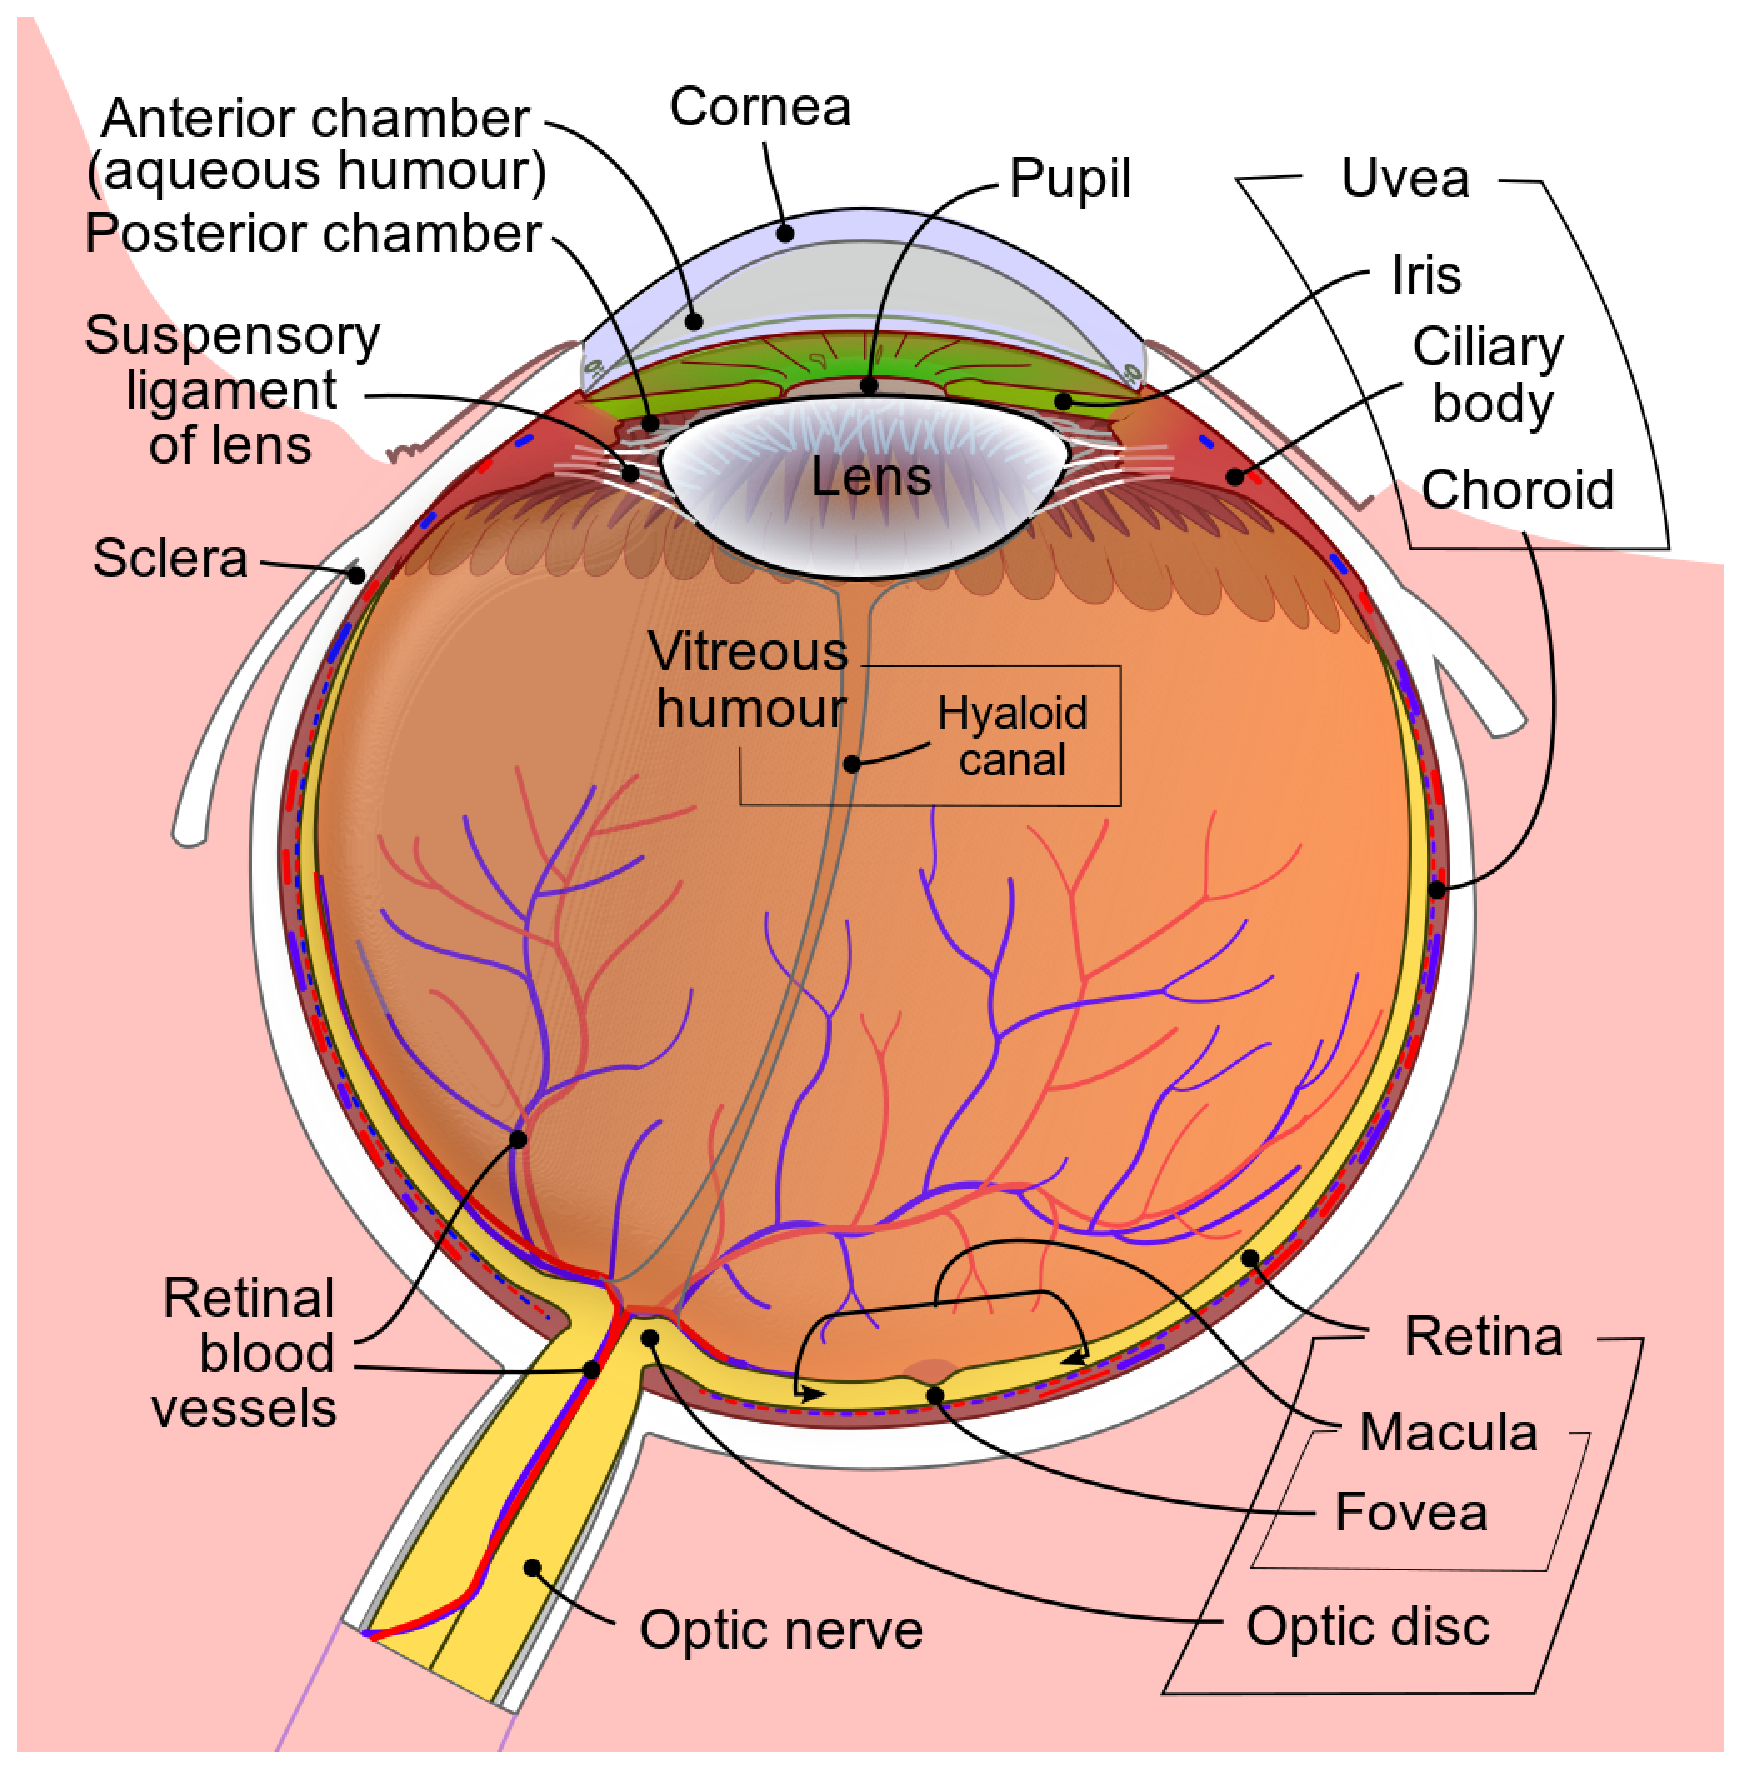
\includegraphics[width=0.8\textwidth]{Figures/chapter_introduction/eye_en.eps}
	\caption[Schematic diagram of the human eye]{Schematic diagram of the human eye (source commons.wikimedia.org)}
	\label{back:fig:eye}
\end{figure}

Diabetes is a disorder of the body due to its inability of producing or responding to the hormone insulin, resulting in abnormal metabolism of carbohydrates and elevated levels of glucose in the blood. Such high blood glucose levels can damage blood vessels and nerves, increasing the probability in diabetic patients of developing other derived diseases, like Diabetic Retinopathy. 

Diabetes can be of two different types: type 1 and 2. Type 1 is an autoimmune disease that causes the insulin producing beta cells in the pancreas to be destroyed, preventing the body from being able to produce enough insulin to adequately regulate blood glucose levels. Because type 1 diabetes causes the loss of insulin production, it therefore requires regular insulin administration. Type 2 is a metabolic disorder that results in hyperglycemia, ie. high blood glucose levels, due to the body either being ineffective at using the insulin it has produced or being unable to produce enough insulin. Type 2 diabetes is characterized by the body being unable to metabolize glucose, leading to high levels of blood glucose, which over time, may damage the organs of the body. \citep{www.diabetes.co.uk}

Diabetic Retinopathy is an associated disease derived from diabetes. It is caused by the damage of the small blood vessels of the retina. Due to diabetes disease related secondary effects, retinal blood vessels can break down, leak or become blocked; affecting the transport of nutrients and oxygen to parts of the retina, causing impaired vision over time. Due to the blockages, abnormal blood vessels can grow on the retina surface, causing an increment of the probability of bleeding and liquid leakages. Such structural changes can result initially in vision blurring and in last stages, even in retinal detachment and/or glaucoma. 

During the first two decades of the diabetes disease, nearly all patients with type 1 and more than 60\% of patients with type 2 diabetes, will develop a retinopathy \citep{fong2004retinopathy}. 

\subsection{Retina health evaluation}

There are several tests that a doctor may perform to evaluate retina eye health:

An \emph{ophtalmoscope} is a specialized type of microscope that allows the inspection of the vitreus, retina and other internal structures of the eye. With this instrument is possible to create a mirrored image of the various portions of the eye.

A \emph{visual field} or \emph{perimetry test}, mesures the ability of the examined eye to see straight ahead and the peripheral vision. The purpose of this test is to determine if there are any peripheral vision areas that are developing blind spots.

\emph{Fluorescein angiography} allows the doctor to inspect retina blood vessels. A vegetable-based dye is injected into patient blood stream. As blood circulates in the retina, a series of quick, sequential photographs of the eye are taken. These photographs provide useful information about its condition. Fluorescein angiography is one of the most important tests performed for determining the diagnosis and treatment of retinal disorders.

\emph{B-scan ultrasound} uses high frequency sound waves to view the back portions of the eye. This technology provides a full surface view of the eye that can be also used for retina condition evaluation.

\emph{Fundus photography} utilizes special cameras to document and track the progress of certain retinal diseases, like diabetic retinopathy, as well as monitor its treatment. This type of images are the used in this thesis for creating the automatic diagnostic system.

\subsubsection{Fundus photography}

Fundus photography is a technique for capturing the internal part of the back of the eye. This technique allows the visualization of main structures present in the back of eye interior, ie. center and peripherical retina, the optic disc and the macula.

Figure \ref{back:fig:fundus_camera} shows a photography of a typical camera used for capturing eye fundus images.

\begin{figure}[ht!]
	\centering
	\includegraphics[width=0.75\textwidth]{Figures/chapter_introduction/fundus_camera.jpg}
	\caption[Typical aspect of a fundus eye camera]{Typical aspect of a fundus eye camera (source commons.wikimedia.org)}  
	\label{back:fig:fundus_camera} 
\end{figure}

Figure \ref{back:fig:fundus_image_left_right_normal} shows an example of the fundus photography of both eyes of a healthy patient. In such images, it can be identified zones like central and peripherical retina, macula (darker part located at the center) and the optic disc (white spherical structure inside the retina).

\begin{figure}[ht!]
	\centering
	\scalebox{1.0}{
		\begin{subfigure}[b]{0.4\textwidth}
			\centering
			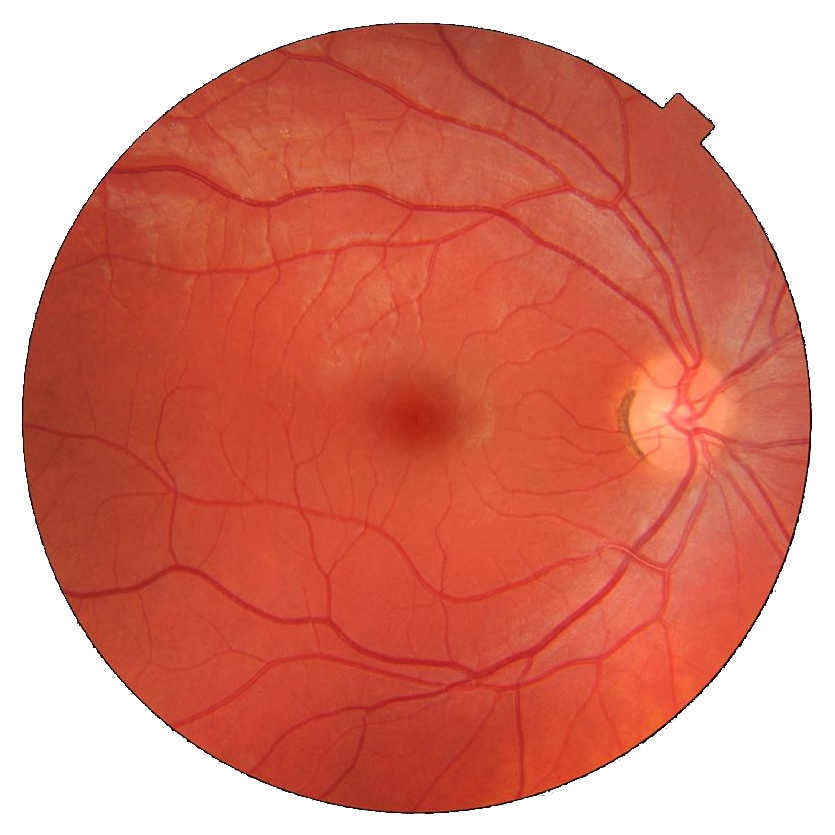
\includegraphics[width=\textwidth]{Figures/chapter_introduction/fundus_normal_eye_right.eps}
		\end{subfigure}
		\hfill    
		\begin{subfigure}[b]{.4\textwidth}
			\centering
			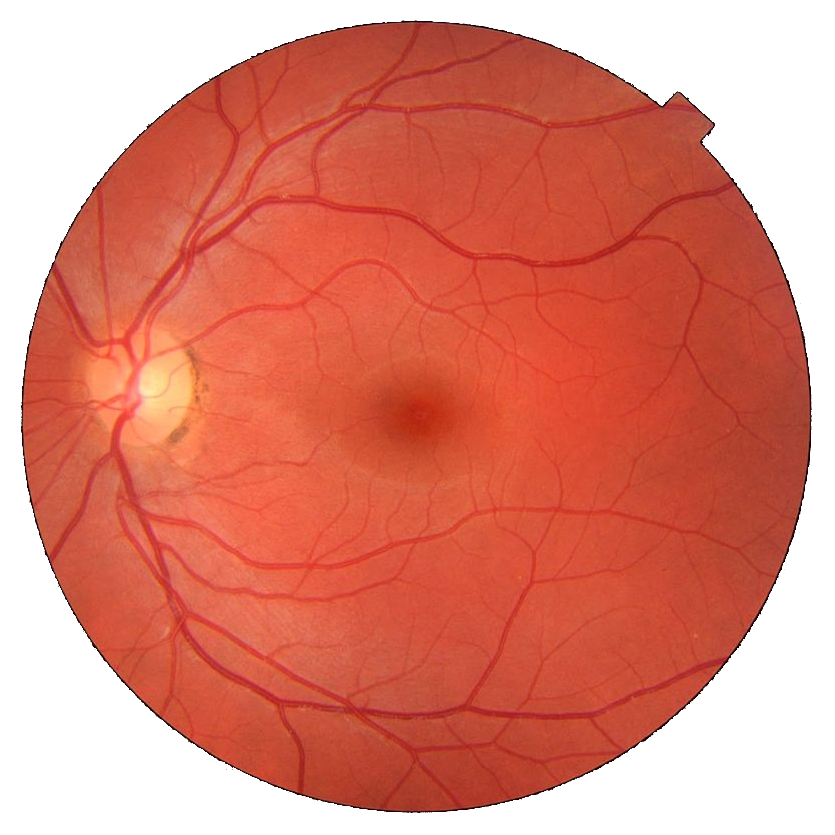
\includegraphics[width=\textwidth]{Figures/chapter_introduction/fundus_normal_eye_left.eps}\\
		\end{subfigure}
	}
	\hfill 
	\caption[Eye fundus images taken from a healthy patient]{Left and right eye fundus images taken from a healthy patient (source commons.wikimedia.org)}  
	\label{back:fig:fundus_image_left_right_normal} 
\end{figure}

With this type of photography is possible to identify, if they exist, the location and type of lesions and to infer from them a diagnostic.

%-----------------------------------
%	SUBSECTION 1
%-----------------------------------
\subsection{Diabetic retinopathy grading and classification}

Accurately grading diabetic retinopathy can be a significant challenge for a untrained person. Medical community establishes a standardized classification based on four severity stages \citep{diaclass} determined by the type and number of lesions (as micro-aneurysms, hemorrhages and exudates) present in the retina: class 0 referring to no apparent Retinopathy, class 1 as a Mild Non-Proliferative Diabetic Retinopathy (NPDR), class 2 as Moderate NPDR, class 3 as a Severe NPDR and class 4 as a Proliferative DR. 

Any of the stages can have no or few symptoms. Therefore, periodic dilated eye examinations are crucial for the detection and evolution study of the disease. Furthermore, diabetic macular edema can develop at any of these stages due to damaged and leaky blood vessels, affecting patient vision quality.

In the following sections diabetic retinopathy disease levels \citep{diaclass} are described:


\subsubsection*{No apparent diabetic retinopathy (class 0)}

The exams done to the fundus images of this class does not show any abnormality, either in the form of micro-aneurysms or in more complex forms. A diabetic patient with no retinopathy has a $<1\%$ chance of developing a PDR in the next four years \citep{klein2009wisconsin}.

\subsubsection*{Mild non-proliferative diabetic retinopathy (class 1)}

This is the earliest stage of the disease. In this stage, micro-aneurysms are the only abnormality found in exams. Class 1 diabetic patients have a $<5\%$ chance of developing a PDR in the next four years \citep{klein2009wisconsin}.

\begin{figure}[ht!]
	\centering
	\includegraphics[width=\textwidth]{Figures/chapter_background/classes/class1.png}
	\caption{Sample image of a Mild NPDR (class 1)} 
	\label{back:fig:class1_sample} 
\end{figure}

Figure \ref{back:fig:class1_sample} shows image EyePACS 11736\_left, tagged as 1 and classified as 1 by our best predictive model. We show lesion map generated by our models described in chapter \ref{Chapter:Interpretation}.

\subsubsection*{Moderate non-proliferative diabetic retinopathy (class 2)}

Moderate NPDR contains dot blot hemorrhages or microaneurysms in at least one quadrant with or without cotton-wool spots, venous beading, or intraretinal microvascular abnormalities (IrMA) but less than the 4:2:1 rule that defines the severe case nd that is explained below.

\begin{figure}[ht!]
	\centering
	\includegraphics[width=\textwidth]{Figures/chapter_background/classes/class2.png}
	\caption{Sample image of a Moderate NPDR (class 2)} 
	\label{back:fig:class2_sample} 
\end{figure}

Figure \ref{back:fig:class2_sample} shows image EyePACS 681\_right, tagged as 2 and classified as 2 by our best predictive model. We show lesion map generated by our models described in chapter \ref{Chapter:Interpretation}.

\subsubsection*{Severe non-proliferative diabetic retinopathy (class 3)}

Exam findings of the severe NPDR are characterized by any of the following cases:

\begin{itemize}
	\item 20 or more intraretinal hemorrhages (dot blot hemorrahages) in each of all four quadrants
	\item Definite venous beading in 2 or more quadrants
	\item Prominent intraretinal microvascular abnormality (IRMA) in one or more quadrants
\end{itemize}

These three points are called the 4:2:1 rule because the abnormalities are required to be present in at least 4, 2 and 1 retina quadrants respectively. Patients with severe NPDR have a $17 \%$ chance of developing high-risk PDR within one year, and $40\%$ chance of high-risk PDR within three years.

\begin{figure}[ht!]
	\centering
	\includegraphics[width=\textwidth]{Figures/chapter_background/classes/class3.png}
	\caption{Sample image of a Severe NPDR (class 3)} 
	\label{back:fig:class3_sample} 
\end{figure}

Figure \ref{back:fig:class3_sample} shows image EyePACS 1561\_left, tagged as 3 and classified as 3 by our best predictive model. We show lesion map generated by our models described in chapter \ref{Chapter:Interpretation}.


\subsubsection*{Proliferative diabetic retinopathy (class 4)}

This is the most advanced stage of the disease. In this stage, new, fragile \& abnormal blood vessels grow on the retina or optic nerve. These blood vessels can leak, affecting vision quality. Exams find either a definite neovascularization, or pre-retinal or vitreous hemorrhages. 
%-----------------------------------
%	SUBSECTION 2
%-----------------------------------

\begin{figure}[ht!]
	\centering
	\includegraphics[width=\textwidth]{Figures/chapter_background/classes/class4.png}
	\caption{Sample image of a PDR (class 4)} 
	\label{back:fig:class4_sample} 
\end{figure}

Figure \ref{back:fig:class4_sample} shows image EyePACS 11854\_left, tagged as 4 and classified as 4 by our best predictive model. We show lesion map generated by our models described in chapter \ref{Chapter:Interpretation}.


\section{Evaluation measures for disease grading}

An objective measure of the classification capabilities of a human or machine system requires the derivation of index measures that enable an exact measure of its performance. Even the most easiest classification task, ie. binary classification, requires the usage of many different indexes to find a good approximation of classification performance. For binary classification, instances of a set are classified as belonging or not to a class. Four possible outcomes can occur: a positive class being correctly classified (true positive, TP), a positive class being incorrectly classified (false positive, FP), a negative class being correctly classified (true negative, TN) and a negative class being incorrectly classified (false negative, FN). Furthermore, the prediction set can be balanced, ie. having the same number of elements of true positive and negative class or can be unbalanced having more instances of one class than another, producing a difference between absolute and relative results. All these variables make difficult to use a unique index for measuring the prediction capabilities. This is the reason why many different indexes exist, even for binary classification. Here below a brief description of the more used indexes for binary classification is presented.

\subsection{Confusion matrix}

The four possible outcomes, defined above, can be represented in a contingency table, known as \emph{confusion matrix}. Table \ref{back:tab:confusion_matrix_example} shows how information is represented in the table. 

\begin{table}[ht]
	\centering
\begin{tabular}{l|l|c|c|c}
	\multicolumn{2}{c}{}&\multicolumn{2}{c}{True class}&\\
	\cline{3-4}
	\multicolumn{2}{c|}{}&Positive&Negative&\multicolumn{1}{c}{Total}\\
	\cline{2-4}
	\multirow{2}{*}{Predicted class}& Positive & $TP$ & $FN$ & $TP+FN$\\
	\cline{2-4}
	& Negative & $FP$ & $TN$ & $FP+TN$\\
	\cline{2-4}
	\multicolumn{1}{c}{} & \multicolumn{1}{c}{Total} & \multicolumn{1}{c}{$TP+FP$} & \multicolumn{    1}{c}{$TN+FN$} & \multicolumn{1}{c}{$Total$}\\
\end{tabular}
	\caption{Binary confusion matrix}
\label{back:tab:confusion_matrix_example} 
\end{table}

Confusion matrix summarizes all information about the problem. All other indexes are derived from the information showed in this table. Confusion matrix can be easily generalized for its usage in multi-class classification cases, just adding as many rows and columns as classes to predict.

\subsection{Sensitivity and Specificity}

Sensitivity and Specificity are the most important indexes derived from confusion matrix.  Sensitivity (eq. \ref{back:eq:sensitivity}), also known as recall, hit rate or true positive rate, measures the proportion of actual positives that are correctly identified as such. Specificity (eq. \ref{back:eq:specificity}), also known as selectivity or true negative rate, measures the proportion of actual negatives that are correctly identified as such. Mathematically is expressed as: .

\begin{equation}
Sensitivity = \frac{TP}{P}
\label{back:eq:sensitivity}
\end{equation}

\begin{equation}
Specificity = \frac{TN}{N}
\label{back:eq:specificity}
\end{equation}

In medical diagnosis, sensitivity measures the model ability to correctly identify those with the disease, whereas specificity measures the model ability to correctly identify those without the disease. 

\subsection{Positive and Negative Predictive Value}

Positive Predictive Value (PPV) (eq. \ref{back:eq:ppv}), also known as precision, measures of the proportion of correctly classified positive cases over the total number of predicted positives. It allows the identification of too conservative models. Negative Predictive Value (NPV) (eq. \ref{back:eq:npv}) measures the same in negative cases.

\begin{equation}
PPV=\frac{TP}{TP+FP}
\label{back:eq:ppv}
\end{equation}

\begin{equation}
NPV=\frac{TN}{TN+FN}
\label{back:eq:npv}
\end{equation}


\subsection{False Positive and Negative Rates}

False Positive Rate (eq. \ref{back:eq:fpr}) and False Negative Rate (eq. \ref{back:eq:fnr}) indexes measure the rate of false values reported by the model. In statistical hypothesis testing these indexes are known as type I and II errors respectively. They are of common use in medical diagnosis, being a very important indexes for defining strategies of screening or testing.

\begin{equation}
FPR=\frac{FP}{N}
\label{back:eq:fpr}
\end{equation}

\begin{equation}
FNR=\frac{FN}{P}
\label{back:eq:fnr}
\end{equation}

\subsection{False Discovery and Omission Rates}

False Discovery Rate (eq. \ref{back:eq:fdr}) measures the proportion false positives which are incorrectly accepted. False omission rate (eq. \ref{back:eq:for}) measures the proportion of false negatives which are incorrectly rejected. Both measures complement FPR and FNR.

\begin{equation}
FDR=\frac{FP}{FP+TP}
\label{back:eq:fdr}
\end{equation}

\begin{equation}
FOR=\frac{FN}{FN+TN}
\label{back:eq:for}
\end{equation}

\subsection{Accuracy}

Accuracy (eq. \ref{back:eq:acc}) measures the proportion of true predictions (positive or negative) over the total of population. This measure can be misleading in unbalanced data sets giving too optimistic results due to the weight of predominant class.

\begin{equation}
ACC=\frac{TP+TN}{Total}
\label{back:eq:acc}
\end{equation}

\subsection{Balanced measures}

Each one of the indexes defined above give a partial information about the classification, this is the reason why a combination of some of them, and not its individual values alone, must be taken into account to make a correct evaluation of model performance. In the quest of finding a unique index that summarizes global performance, a set of meta-indexes have been proposed. These meta-indexes combine the information given by a set of indexes to, in this way, give a unique index with an overall performance evaluation. In between these indexes are: $F_\beta$, Matthews correlation coefficient (MCC) \citep{sammut2011encyclopedia}.

\paragraph{$F_\beta$} (eq. \ref{back:eq:f_measure}) is an harmonic mean between specificity and sensitivity. $\beta$ is a constant that allows to weight the relative importance of both components. For giving the same importance to both variables, $\beta$ is set to 1. 

\begin{equation}
F_\beta = (1 + \beta^2) \frac{sensitivity \cdot specificity}{\beta^2 \cdot specificity + sensitivity}
\label{back:eq:f_measure}
\end{equation}

\paragraph{MCC} (eq. \ref{back:eq:mcc}) acts as a correlation coefficient between observed and predicted values. MCC is related to the chi-square statistic for a 2x2 contingency table. 

\begin{equation}
MCC = \frac{TP \cdot TN + FP \cdot FN}{\sqrt{(TP \cdot FP)(TP \cdot FN) (TN \cdot FP)(TN \cdot FN)}}
\label{back:eq:mcc}
\end{equation}


\subsection{The Kappa family of statistics}

Ordinal Regression is a particular case of multi-class classification where an ordering of the classes can be established a priori, based on some underlying properties present in data.

In medical diagnosis, it is a typical situation the use of an ordinal or nominal classification scale for defining the severity of patient diseases. Frequently, such scales are designed for identifying the gradation of disease level from mild cases to the most severe, being then a particular case of an ordinal regression.

A typical situation in the definition of such gradation classes is the inherent existence of some subjectivity. Normally, the underlying properties that define the classification are not completely observable or cannot be completely identified, causing even experts to differ to some extent in its conclusions, requiring the usage of an index that allows the objective measure of the level of agreement between experts.

Kappa family of statistics \citep{sim2005kappa} are a way of measuring such inter-rater and intra-rater agreement, ie. diagnostics reliability. Main purpose of the kappa derived statistics is to measure of "true" agreement. When a set of experts evaluate a fact, there are mainly to sources of possible agreement: one coming from expertise and another from chance. Kappa index discounts the probability of agreement by chance, being then a pure measure of "true" agreement.

In its binary classification form and for evaluation of two experts, kappa can be expressed as eq. \ref{back:eq:kappa_bin}.

\begin{equation}
\kappa = \frac{P_o - P_c}{1 - P_c}
\label{back:eq:kappa_bin}
\end{equation}

being $P_o$ the proportion of observed agreement and $P_c$ the proportion of agreement by chance. The range of possible values of kappa is of -1 to +1. Denoting $\kappa=-1$ complete disagreement, $\kappa=0$ random agreement and $\kappa=+1$ complete agreement between raters.

\paragraph{Kappa for multi-class classification.} Kappa coefficient can be extended for its use with more than 2 ordinal categories. When more than two classes are present, disagreement can be expressed by the distance between predictions of both raters. Weighted kappa is the multi-class version of original kappa, where the discrepancy is penalized by a weight that is a function of the distance between both predictions. The most common weight strategy used is the quadratic, where weights used are proportional to the square of the distance between predictions of both raters. In such case, the index is known as \emph{Quadratic Weighted Kappa}, QWK or $\kappa$ indistinctly \citep{cohen1968weighted}. This index is the most commonly used by medical community and it is the main one used in this thesis for performance evaluation.

\begin{equation}
\kappa = \frac{\sum \omega f_o - \omega f_c}{n - \sum \omega f_c}
%\kappa = 1 - \frac{\sum_{i,j} \omega_{i,j} P_{i,j}}{\sum_{i,j} \omega_{i,j} E_{i,j}}
\label{back:eq:kappa_qwk}
\end{equation}

Equation \ref{back:eq:kappa_qwk} shows the expression of quadratic weighted kappa, where $\sum \omega f_o$ is the sum of weighted observed frequencies in the confusion matrix cells, and $\sum \omega f_c$ the sum of weighted frequencies expected by chance in the confusion matrix cells. In case of using linear weights, $\omega = 1 - \frac{|i-j|}{k-1}$ and in case of quadratic weights, $\omega = 1 - \big( \frac{i-j}{k-1} \big)^2$.  %Being $\omega_{i,j}$ the weight applied to the proportion of predictions rated by first rater as $i$ and for second rater as $j$ that, by definition is equal to $\omega_{i,j} = (i - j)^2$. 

Alternatively, QWK can be defined in terms of observation and expectation histogram matrices. For $N$ classes, a NxN observation matrix $O$ is constructed, such that $O_{i,j}$ correspond to the number of elements rated as class $i$ by rater 1 and as class $j$ by rater 2. A NxN expectation matrix $E$ is also calculated as the outer product between each rater's histogram vector, normalized such that $E$ and $O$ have the same sum. Representing the weights as $\omega = \frac{(i-j)^2}{(N-1)^2}$, kappa can be calculated as:

\begin{equation}
\kappa = 1 - \frac{\sum_{i,j} \omega_{i,j} O_{i,j}}{\sum_{i,j} \omega_{i,j} E_{i,j}}
\label{back:eq:kappa_qwk2}
\end{equation}

\paragraph{Kappa interpretation.} In \citep{landis1977measurement} the next standards of agreement are proposed: $\kappa \leq 0$ indicating poor agreement, $0.01 \leq \kappa \leq 0.20$ slight, $0.21 \leq \kappa \leq 0.40$ fair, $0.41 \leq \kappa \leq 0.60$ moderate, $0.61 \leq \kappa \leq 0.80$ substantial and $\kappa \geq 0.81$ almost perfect. Value of $kappa$ is influenced by the weighting applied and by the number of classes, bias and prevalence, this is the reason why kappa values are not comparable across variables having different prevalence or bias \citep{sim2005kappa}. In the case of diabetic retinopathy disease grading, using QWK, the inter-rating agreement between expert ophthalmologists is about $0.80$. For the purpose of this thesis, such value ($\kappa = 0.80$) is the standard of reference our models are compared against.

\subsection{How to define human performance}

A key factor for evaluation of machine performance against humans is the standard used to measure the last one. In the context of medical classification, the next comparison standards can be used:

\begin{enumerate}
\item A person (not a doctor)
\item A general doctor
\item A specialized doctor
\item A highly experienced specialized doctor
\item A team of highly experienced specialized doctors
\end{enumerate}

The team of highly experienced specialized doctors can be approximated to the \emph{Bayes Optimal Error} \citep{fukunaga2013introduction}, \citep{tumer1996estimating}. In any case, it is important to define the standard we are comparing against. For the purpose of this thesis, human performance is established as the given by a \emph{highly experienced specialized doctor}.

\section{Machine Learning}

Machine Learning is a Computer Science discipline, sub-field of Artificial Intelligence, that include all the tools and techniques used for enabling computers to learn from data and, from a more ambitious perspective, giving computers the ability of acting without being explicitly programmed.  

All tools and techniques available in the discipline can be classified according on the type of learning algorithm that they implement: supervised, unsupervised and reinforced learning.

\paragraph{Supervised learning} algorithms require all the instances of the training set to be labeled. From this previous knowledge the algorithm is able to learn and generalize, being able to predict new never seen before samples. From a probability perspective these type of algorithms learn a conditional distribution, ie. $P(c|X)$, being $c$ the class to predict and $X$ the sample.

\paragraph{Unsupervised learning} algorithms allow the learning of underlying regularities present in the training set without requiring labeling of the individual instances. From a probability perspective, such models are able to learn the joint distribution of the population represented by the training set, ie. $P(X)$, being $X$ the sample.

\paragraph{Reinforcement learning} algorithms give models the capacity of learning from environment, ie. accumulating experience from its interaction with the surroundings. Such models are goal oriented,  having an internal representation of the environment that is updated periodically with the objective of maximizing gain.

\subsection{Supervised Learning}

In this thesis we used supervised learning techniques for learning from data. As previously stated, in this learning paradigm a \emph{labeled training set} is used as a foundation for learning general representations that can be used for generalizing behaviors and inferring then new labels in never seen before data.

\subsubsection{Classification vs Regression}

The objective of supervised learning is the learning of a conditional probability distribution in the form of $P(c|X)$. Depending on the nature of the variable to be predicted, it can be differentiated between classification or regression. Fundamentally, classification is about a disjoint class label prediction and regression is about a quantity prediction. Ordinal regression is a particular case of classification, where some a priori class ordinality can be established.

\subsubsection{Dataset management}

In supervised learning, the source of knowledge is represented by a labeled data set. The probability distribution of the population that it is supposed to be predicted is assumed to be represented by a sample, ie. a labeled data set. The design process of a predictive model has two parts: building the model (ie. training) and statistical evaluation of its performance. Performance evaluation require the usage of a never seen before data set, so the original full data set is required to be split in two parts: one for training (called \emph{training set}) and another for testing (called \emph{test set}). Both train and test set must be big enough either for training good models or for having a high statistical confidence of its generalization capabilities.

\subsubsection{Strategies for hyper-parameter optimization}

Frequently, supervised learning models have parameters that must be fixed before learning. In such cases, model performance can change dramatically depending on the selected parameters, requiring also a meta-learning parameter optimization for selection of the highest performance model, more commonly known as hyper-parameter optimization. 

Different strategies can be followed in order to optimize such meta-parameters:

\paragraph{Hold Out method:} This method splits original training data set using random sampling without repetition into 2 subsets. The first called training set is used for fitting the model/s, the second one, called validation set is used for hyper-parameter optimization and for model selection, not only between hyper-parameters but also between different types of models. As a rule of thumb, training set use to have between 50\% to 70\% of the data and validation set between 50\% to 30\%.

\paragraph{K-fold cross validation:} The original training set is split in $K$ folds of the same size using random sampling without repetition. The model/s are trained $K$ times, each one of them using as training set $K-1$ folds and $1$ (the not used one) as a validation set. Prediction error is the average of $K$ individual errors. Error variance can be used as a measure of the model stability. The advantage of this method is that it matters less how the data is divided, ie. the model is less prone of having selection bias. After choosing the best model hyper-parameters and/or model, a retrain with the whole data set is recommended.

\paragraph{Leave one out cross-validation:} It is a type of K-fold cross validation where it is hold out only one sample each time. It is a good way to validate, but requires a high computation time.

\paragraph{Bootstrap methods:} It randomly draws data sets from the original sample. Each sample size is equal to the original training size. Each model/s with its particular hyper-parameters is fitted using the bootstrapped samples. Model/s are examined with the out-of-bag data, ie. data not selected in each bootstrap.

\subsection{Algorithms used in supervised machine learning}

The most widely used learning algorithms can be divided into the next categories:

\begin{itemize}
\item Linear / Logistic regression
\item Support Vector Machines
\item Probabilistic Graphical Models
\item Decision trees related algorithms
\item Deep Learning (Multilayer Perceptron, Neural Networks)
\item Others (clustering, association rules, inductive logic, representation learning, similarity and metric learning, sparse dictionary learning, genetic algorithms, etc.)
\end{itemize}

\paragraph{Linear/Logistic Regression} are regression and classification algorithms, where a linear combination of the inputs is optimized for least squares error minimization in the first case and for cross entropy minimization in the second.

\paragraph{Support Vector Machines} are similar to linear/logistic regression but using a different optimization function. They minimize the Hinge loss, giving as a result maximum-margin classifiers. Support vector machines can be used as linear classifiers but also as a non-linear ones, substituting its features with so-called kernels, that are non-linear functions of the features and training set samples. 

\paragraph{Probabilistic Graphical Models} are a set of models based on probabilistic conditional dependency graphs that use bayesian rules for model construction and inference.

\paragraph{Decision Trees based models} are a set of very effective algorithms based on the usage of weak learners like decision trees for constructing very powerful predictors combining them using bagging or boosting techniques. This category include algorithms like Random Forest or Gradient Boosting.

\paragraph{Deep Learning} also known as Artificial Neural Networks or Multilayer Perceptrons, is a set of Machine Learning techniques for automatically constructing models from the underlying distribution represented by a large set of examples, using multiple levels of representation (in the form of layers), with the final objective of mapping a high-multidimensional input into a smaller multidimensional output (f: $\mathbb{R}^{n} \mapsto \mathbb{R}^{m}, n \gg m$). This mapping allows the classification of multidimensional objects into a small number of categories. The model is composed by many neurons that are organized in layers and blocks of layers, using a cascade of layers in a hierarchical way. Every neuron receives the input from a predefined set of neurons. Every connection has a parameter that corresponds to the weight of the connection. The function of every neuron is to make a transformation of the received inputs into a calculated output value. For every incoming connection, the weight is multiplied by the input value received by the neuron and the aggregated value that used by an activation function that calculates the output of the neuron. Parameters are usually optimized using a stochastic gradient descent algorithm that minimizes a predefined loss function. Network parameters are updated after back-propagating the loss function gradients through the network. These hierarchical models are able to learn multiple levels of representation that correspond to different levels of abstraction, which enables the representation of complex concepts in a compressed way \citep{nature-deep-learning}, \citep{888}, \citep{Bengio:2013:RLR:2498740.2498889}, \citep{bengio-2009}. The models used in this thesis are based mainly in Deep Learning.

\subsection{Pattern recognition}

\subsubsection{Traditional models of pattern recognition}

The traditional model for pattern recognition since the 50's were based on a fix design of a set of important features manually engineered or derived from a fixed kernel (Fig. \ref{back:fig:trad_pat_rec}). Such kernels allowed the extraction of texture, statistic, position, geometry features that were posteriously combined with a simple classifier. A great diversity of methods for feature extraction exist as the local binary pattern, histogram of oriented gradients, gray level co-occurence matrix, gabor filters, between others. In the classification phase it was common practice to use k-nearest neighbors, linear discriminant analysis, support vector machines or decision trees derived algorithms like random forest or gradient boosting.

\begin{figure}[!h]
	\centering
	\smartdiagramset{back arrow disabled=true}
	\resizebox{.9\linewidth}{!}{\smartdiagram[flow diagram:horizontal]{Image Input, Hand-Crafted Feature Extractor, 'Simple'\\Classifier, Class}}
	\caption{Traditional pattern recognition scheme}
	\label{back:fig:trad_pat_rec}
\end{figure}

Such pattern recognition pipeline required a lot of labor time for designing the appropriate filters for every particular application.

\subsubsection{Deep Learning for pattern recognition}

Deep learning for pattern recognition represents a change of the design paradigm. Instead of hand-crafting features, a fully trainable model is designed, that is the combination of a trainable feature extractor and a trainable classifier (Fig \ref{back:fig:dl_pat_rec}), creating a end-to-end automatic learner.

\begin{figure}[!h]
	\centering
	\smartdiagramset{back arrow disabled=true}
	\resizebox{.9\linewidth}{!}{\smartdiagram[flow diagram:horizontal]{Image Input, Trainable Feature Extractor, Trainable Classifier, Class}}
	\caption[Deep Learning pattern recognition scheme]{Deep Learning pattern recognition scheme (end-to-end learning)}
	\label{back:fig:dl_pat_rec}
\end{figure}

\subsubsection{Types of Deep Learning architectures}

Neural networks are the architectures lying under the term of deep learning. They are directed graphical models with a defined architecture formed by their building block, the neuron. We can differentiate between three typical base architectures: fully connected, convolutional and recurrent neural networks. Every designed network can be classified into one of such architectures or as combinations of them. Each one is suitable for different types of problems. Recurrent neural networks are optimized to be used for serially organized information, for example text or sound related problems. Convolutional neural networks are designed for local correlation exploitation, for example in the case of images. Fully connected layers are designed to be used in cases where all the information is equally important, for example in classification layers. The models designed in this thesis use mainly convolutional neural networks.

\subsubsection{Convolutional neural networks}

Convolutional neural networks (fig. \ref{back:fig:cnn}), firstly proposed successfully in \citep{lecun1989backpropagation} for handwritten image recognition, are the main type of network used in this thesis for diabetic retinopathy image classification and interpretation.

\begin{figure}[!htb]
	\centering
	\includegraphics[width=0.9\textwidth]{Figures/chapter_background/typical_cnn.png}
	\caption[High level representation of a typical convolutional neural network]{High level representation of a typical convolutional neural network (source: commons.wikimedia.org)}
	\label{back:fig:cnn}
\end{figure}

CNNs are a type of neural network specialized in exploiting the natural local correlations present in images. They are able to create local abstractions that are combined layer-by-layer forming more elaborated meta-abstractions, hopefully, being able to disentangle the information contained in the image, forming features that are useful for solving a particular classification/regression problem. 

As conventional neural networks, they are formed by a set of layers that are piled together. Each layer has a convolutional operator that allows the transformation of a input tensor into another one. The output tensor can pass through other transformations inside the same layer, like a batch-normalization, an activation function or reducing size functions like max-pooling or average pooling blocks. All these functions are parametric, ie. they have learnable parameters, that are tuned through a loss function optimization process with the objective of enhancing the classification/regression capabilities of the network. The characteristic building block of such type of network is the convolution operator.

\paragraph{Convolution operator} (fig. \ref{back:fig:convolution_operator}) is repeatedly applied to different localizations of the input. Parameters that define such operator are: a tensor of \emph{number of feature inputs x convolution width x convolution height x number of outputs}, \emph{horizontal and vertical padding} and \emph{horizontal and vertical stride}. Padding defines the number of pixels that must be added to the width and height of the input before applying it, ie. if the input has a \emph{width x height} original size, is extended for applying the operator to \emph{(width + 2 x padding width) x (height + 2 x padding height)}. The operator is applied in every location of the input with a separation between initial points of \emph{horizontal stride} and \emph{vertical stride}. The output value correspond to the linear combination of the convolution parameters with input values.

\begin{figure}[!ht]
	\centering
	\begin{subfigure}{0.2\textwidth}
		\includegraphics[scale=0.5]{Figures/chapter_background/convolution_operator/padding_strides_odd_00.pdf}
	\end{subfigure}
	~ % spacing  ~, \quad, \qquad
	\begin{subfigure}{0.2\textwidth}
	\includegraphics[scale=0.5]{Figures/chapter_background/convolution_operator/padding_strides_odd_01.pdf}
	\end{subfigure}
	~ % spacing  ~, \quad, \qquad
	\begin{subfigure}{0.2\textwidth}
	\includegraphics[scale=0.5]{Figures/chapter_background/convolution_operator/padding_strides_odd_02.pdf}
	\end{subfigure}
	~ % spacing  ~, \quad, \qquad
	\begin{subfigure}{0.2\textwidth}
	\includegraphics[scale=0.5]{Figures/chapter_background/convolution_operator/padding_strides_odd_03.pdf}
	\end{subfigure}
	\caption[Convolution operator of 3x3, stride 2, padding 1]{Convolution operator of 3x3 with stride 2 and padding 1 in both directions applied to a 6x6 input. Only one input and output features are shown \citep{dumoulin2016guide}.}
	\label{back:fig:convolution_operator}
\end{figure}

\paragraph{Pooling operators} (fig. \ref{back:fig:pooling_operator}) are other typical elements used in CNNs. They are used for reducing the size of feature maps. Max-pooling operators select from a predefined window the maximum value and discards the others. Average-pooling, selects the average. Both, are the most common strategies for reducing the size of feature maps.

\begin{figure}[!ht]
	\centering
	\begin{subfigure}{0.2\textwidth}
		\includegraphics[scale=0.5]{Figures/chapter_background/max_pooling/numerical_max_pooling_05.pdf}
	\end{subfigure}
	~ % spacing  ~, \quad, \qquad
	\begin{subfigure}{0.2\textwidth}
		\includegraphics[scale=0.5]{Figures/chapter_background/max_pooling/numerical_max_pooling_06.pdf}
	\end{subfigure}
	~ % spacing  ~, \quad, \qquad
	\begin{subfigure}{0.2\textwidth}
		\includegraphics[scale=0.5]{Figures/chapter_background/max_pooling/numerical_max_pooling_07.pdf}
	\end{subfigure}
	~ % spacing  ~, \quad, \qquad
	\begin{subfigure}{0.2\textwidth}
		\includegraphics[scale=0.5]{Figures/chapter_background/max_pooling/numerical_max_pooling_08.pdf}
	\end{subfigure}
	\caption[Max-pooling operator of 3x3, stride 1, padding 0]{Max-pooling operator of 3x3 with stride 1 and padding 0 in both directions applied to a 5x5 input. Only one input and output features are shown \citep{dumoulin2016guide}.}
	\label{back:fig:pooling_operator}
\end{figure}

\paragraph{Batch normalization} are another typical element used in CNN layers. It applies a normalization to the inputs that help to reduce covariate shift, increasing stability and acting as a regularizer \citep{batch-norm}.

\paragraph{Activation function} (fig. \ref{back:fig:activations}) is a key element of neural networks. ReLU is the most versatile, stable and used one. Sigmoid function, the most used one in the 80's, only used nowadays for certain types of output layers, due to its gradient descent vanishing problems. Without them, deep learning models would behave just like linear functions. In the 80s the most used activation function was the sigmoid, a smooth non-linear function, that is continously differentiable. Despite its interesting properties, it has a very important concern, called gradient vanishing problem \citep{glorot2010understanding}. Sigmoid first derivative becomes flat not far from the origin, affecting network loss optimization due to near-to-zero gradients. In \citep{nair2010rectified} ReLUs were used for improving Restricted Boltzmann Machines (RBMs), approximating stepped sigmoid units with ReLUs. In \citep{glorot2011deep} the authors compared the performance of Sigmoid, Tanh and ReLU arriving to the conclusion that despite Sigmoid being more plausible biologically, Tanh and ReLU were more suitable to be used as activation function for training multi-layer perceptrons. ReLU networks have better performance in general, despite its non-differentiability at zero and its hard non-linearity. Furthermore, ReLU networks lead to sparse representations, being beneficial, both because information is represented in a more robust manner and because it leads to significant computational efficiency. Moreover, the simplicity of the function and its derivative reduces calculation time, being of significant importance when working with big networks. The constant value of the gradient, helps avoiding the gradient vanishing problem, allowing the design of deeper networks. For then on, ReLU has become the default activation function for deep learning. Many other activation functions have been published, like LeakyReLU, but not introducing significant performance gains.

\begin{figure}[h!]
	\centering
	\begin{subfigure}{0.2\textwidth}
		\includegraphics[scale=0.6]{Figures/chapter_background/activation_functions/relu.pdf}
		\caption{ReLU}
	\end{subfigure} ~
	\begin{subfigure}{0.2\textwidth}
		\includegraphics[scale=0.6]{Figures/chapter_background/activation_functions/leakyrelu.pdf}
		\caption{leakyrelu}
	\end{subfigure} ~
	\begin{subfigure}{0.2\textwidth}
		\includegraphics[scale=0.6]{Figures/chapter_background/activation_functions/tanh.pdf}
		\caption{Tanh}
	\end{subfigure} ~
	\begin{subfigure}{0.2\textwidth}
		\includegraphics[scale=0.6]{Figures/chapter_background/activation_functions/sigmoid.pdf}
		\caption{Sigmoid}
	\end{subfigure}
	\caption{Typical activation functions used in Deep Learning}
	\label{back:fig:activations}
\end{figure}

\paragraph{Typical CNN architectures.} CNNs have been demonstrated to be very effective in solving complex classification, detection and segmentation problems. Table \ref{back:fig:imagenet_models} shows a summary of the most successful Imagenet \citep{imagenet_cvpr09} prediction standardized architectures sorted by its performance solving the complex Imagenet classification task. The more successful network presented in the table is \emph{InceptionResNetV2} having more than 55 million of parameters. \emph{Xception} has a similar accuracy using less than a half of parameters. \emph{MobileNetV2}, an architecture designed to be used in mobile devices, with only 3.4 million of parameters has an accuracy similar to the achieved with older architectures as \emph{VGG16} and \emph{VGG19}, that used more than 100 million of parameters.

\begin{table}[h!]
	\centering
	\scalebox{0.55} {
	\begin{tabular}{lccccccc}
		\textbf{Model}    & \textbf{Input size} & \textbf{\shortstack{Imagenet\\Top-1\\Accuracy}} & \textbf{Params} & \textbf{Depth} & \textbf{Residual} & \textbf{Publication} & \textbf{Source} \\
		\hline
		InceptionResNetV2 & (299,299,3)         & 0.804                            & 55.9M               & 572            & Yes               & 2016-02              & \citep{szegedy2017inception}          \\
		InceptionV4       & (299,299,3)         & 0.802                            & 55.9M               &                & No                & 2016-02              & \citep{szegedy2017inception}          \\
		Xception          & (299,299,3)         & 0.790                            & 22.9M               & 126            & Yes               & 2016-10              & \citep{chollet2017xception}          \\
		InceptionV3       & (299,299,3)         & 0.788                            & 23.8M               & 159            & No                & 2015-12              & \citep{szegedy2016rethinking}          \\
		DenseNet201       & (224,224,3)         & 0.770                            & 20.2M               & 201            & Dense             & 2016-08              & \citep{huang2017densely}        \\
		ResNet50          & (224,224,3)         & 0.759                            & 25.6M               & 168            & Yes               & 2015-12              & \citep{he2016deep}       \\
		DenseNet169       & (224,224,3)         & 0.759                            & 14.3M               & 169            & Dense             & 2016-08              & \citep{huang2017densely}        \\
		MobileNetV2 (1.4) & (224,224,3)         & 0.747                            & 6.9M                &                & Yes               & 2018-01              & \citep{sandler2018mobilenetv2}          \\
		DenseNet121       & (224,224,3)         & 0.745                            & 8M                  & 121            & Dense             & 2016-08              & \citep{huang2017densely}        \\
		VGG19             & (224,224,3)         & 0.727                            & 143.7M              & 26             & No                & 2014-09              & \citep{vggnet}          \\
		MobileNetV2       & (224,224,3)         & 0,720                            & 3.4M                &                & Yes               & 2018-01              & \citep{sandler2018mobilenetv2}          \\
		VGG16             & (224,224,3)         & 0,715                            & 138.3M              & 23             & No                & 2014-09              & \citep{vggnet}          \\
		MobileNetV1       & (224,224,3)         & 0.706                            & 4.2M                &                & Yes               & 2017-06              & \citep{howard2017mobilenets}          \\
		SqueezeNet        & (227,227,3)         & 0.575                            & 1.2M                &                & Yes               & 2016-02              & \citep{iandola2016squeezenet}       \\
		AlexNet           & (227,227,3)         & 0.571                            & 62M                 & 8              & No                & 2012-00              & \citep{NIPS2012_4824}           
	\end{tabular}
}
\caption{List of the most successful classification architectures used for Imagenet prediction}
\label{back:fig:imagenet_models}
\end{table}


\subsection{Prediction error: bias vs variance}

Prediction error has two sources of error: bias and variance.
\emph{Bias} is the difference between expected average prediction and the real value. \emph{Variance} is a measure of the model variability prediction for a given data point. Figure \ref{back:fig:bias_variance} show visual examples of different scenarios of bias and variance combinations.

\begin{figure}[h!]
	\centering
	\includegraphics[width=0.50\textwidth]{Figures/chapter_background/bias_variance.png}
	\caption{Bias vs Variance extreme possible scenarios}
	\label{back:fig:bias_variance}
\end{figure}

A low bias - high variance model gives predictions where its expected average is near the true value, but its individual predictions are highly dispersed around the true value. A high bias - low variance model gives predictions far from the true value but with small variability between the predictions. A high bias - high variance model gives predictions far from the true value and with high variability between them. Finally a low bias - low variance model is the best one having close to the true value predictions and low variability between individual predictions.

\subsection{Model ensembling}

Model ensembling \citep{zhou2012ensemble} is a way of improving accuracy of predictions using a combination of classifiers that are trained using different models, data, hyper-parameters or parameter initializations. Every difference introduced in the ensembling increases diversity and improves generalization capabilities of final model. The drawbacks are loss of interpretability and the increase in complexity of evaluation of ensembled model. 

Classifiers can be combined using different techniques: bagging, boosting and model stacking.

\paragraph{Bagging:} Bagging uses a base predictor, ie. a weak learner, for creating a pool of N weak predictors. Every predictor is generated using a random sampling with replacement from the original dataset. In the classifier phase, all predictions are averaged (regression) or selected by majority vote (classification). Model predictions obtained have lower variance than the coming from original predictors.

\paragraph{Boosting:} Boosting predictor generation process is sequential, building multiple incremental models to decrease bias, while keeping variance small. In every step, Boosting increases the weights of miss-classified data to emphasize the importance of the most difficult cases. Boosting also assigns weights in the classification stage to predictors giving more importance to best predictors. Due to this weighting strategy, boosting is able not only to reduce variance but also to reduce bias. In counterpart, boosting can over-fit training data, problem that is not present in bagging predictors.

\paragraph{Model stacking:} allows the combination of model predictors of completely different nature. It fits a meta-model such as for example, a logistic regression, using cross validation predictions coming from multiple models, achieving better results than source predictors.


\section{Data}

Data is at the core of any machine learning model, its quality determines the validity and generalization capabilities of any model derived from it. Machine learning paradigm is based, precisely, in the design of models that are able to learn from data. In this section, we aim to make an exploratory analysis of the data sets that have been used for the elaboration of this thesis. 

\subsection{Datasets}

Three different datasets have been used: EyePACS, Messidor-2 and Reus. EyePACS, the biggest dataset available, have been used for model training, validation and testing. Messidor-2 and Reus have been used for testing purposes and for checking validity of trained models over alternative populations.

\subsection{EyePACS dataset}\label{dataset:eyepacs}

EyePACS dataset \citep{eyepacs_kaggle} is formed by the images of $44,346$ different patients. For each one of them, left and right eye images are available, having a total of $88,692$ retina fundus images. Each one of the images is classified according to the standards defined in \citep{diaclass}. The images are taken in variable conditions: by different cameras, in different illumination conditions and have different resolutions. The dataset is highly imbalanced having $65,343$ class 0 images; $6,195$ of class 1; $13,153$ of class 2; $2,087$ of class 3 and $1,914$ of class 4. Figure \ref{back:fig:eyepacs_pie} shows a graphical representation of the class distribution of the dataset.

\subsection{Messidor-2 dataset}\label{dataset:mesidor2}

Messidor-2 dataset \citep{decenciere_feedback_2014} is formed by a total of $1,748$ retina fundus images. Each one of the images has adjudicated grades for Diabetic Retinopathy Severity following \citep{diaclass}, Diabetic Macular Edema (DME) based on hard exudates classification, and Gradability. The grades were adjudicated by a panel of three Retina Specialists \citep{google_brain_messidor2}. This fact gives high confidence to the tagging (being near Bayes Optimal Error), making the dataset suitable to be used as a high confidence test set. The dataset is also highly imbalanced having $1,017$ class 0 images; $270$ of class 1; $347$ of class 2; $75$ of class 3 and $35$ of class 4. No explicit differentiation between eyes of the same patient is given. Figure \ref{back:fig:messidor2_pie} shows a graphical representation of its class distribution.

\subsection{HUSJR dataset}\label{dataset:reus}

We have been able to obtain a third dataset from a reference hospital in Catalonia region: Hospital Universitari Sant Joan de Reus (HUSJR). It is located in Tarragona province, concretely in the city of Reus. The ophthalmology unit of this hospital has collected data from population of Caucasian, T2DM patients between January 1, 2007 and December 31, 2016. This included 85.33\% of T2DM patients of this area. Patients have been screened with the nonmydriatic fundus camera units (NMCU) at HUSJR. Screening was carried out with one 45º field retinography, centered on the fovea. If DR was diagnosed, the patient was sent to the Ophthalmology service at our hospital and another 2 retinographs of 45º were taken according to EURODIAB guidelines \citep{aldington1995methodology}.

This dataset is used in chapter \ref{Chapter:Inference} for evaluation of the performance of designed models. It consist of $19,230$ tagged retinograhies: $15,123$ with no apparent DR, $2,576$ with mild DR, $944$ with moderate DR and $587$ with severe proliferative or non-proliferative DR. This dataset has a higher number of the most severe cases of the disease, allowing the extraction of finer statistical measures is such cases. In this dataset, no differentiation between class 3 and class 4 is given, considering that they belong to the same class 3. Figure \ref{back:fig:reus_pie} shows a graphical representation of its class distribution. Figure \ref{back:fig:reus_pie} shows a graphical representation of its class distribution.

\begin{figure}[h]
	\centering
	\begin{subfigure}[b]{0.3\textwidth}
		\centering
		\scalebox{0.5}{
		\begin{tikzpicture}[scale=0.1]
		\pie[cloud, text=inside,scale font, radius=30]
		{
			73.7/Class 0,
			7.0/Class 1,
			14.8/Class 2,
			2.3/Class 3,
			2.2/Class 4
		}
		\end{tikzpicture}
		}
		\caption{EyePACS}\label{back:fig:eyepacs_pie}
	\end{subfigure}
	\begin{subfigure}[b]{0.3\textwidth}
	\centering
		\scalebox{0.5}{
		\begin{tikzpicture}[scale=0.1]
		\pie[cloud, text=inside,scale font, radius=30]
		{
			58.2/Class 0,
			15.5/Class 1,
			19.9/Class 2,
			4.4/Class 3,
			2.0/Class 4
		}
		\end{tikzpicture}
	}
	\caption{Messidor-2}\label{back:fig:messidor2_pie}
	\end{subfigure}
	\begin{subfigure}[b]{0.3\textwidth}
	\centering
	\scalebox{0.5}{
		\begin{tikzpicture}[scale=0.1]
		\pie[cloud, text=inside,scale font, radius=30]
		{
			78.6/Class 0,
			13.4/Class 1,
			4.9/Class 2,
			3.1/Class 3
		}
		\end{tikzpicture}
	}
	\caption{HUSJR}\label{back:fig:reus_pie}
	\end{subfigure}
	\caption{Datasets class percentage distribution}  
	\label{back:fig:datasets_class_percentage} 
\end{figure}

\section{Summary of the data and methods used in this thesis}

All classification and interpretation models used in this thesis are based on convolutional neural networks. For its optimization, different loss functions are used, including a new contribution for ordinal regression based on the quadratic weighted kappa (see chapter \ref{Chapter:QWK_loss}). Ensembling methods are also used for obtaining better predictions, based either on averaging different rotated versions of the same image or on bayesian inference (see chapter \ref{Chapter:Classification}). As a evaluation function we use mainly quadratic weighted kappa. 

Relating to data, all models are trained using different subsets of EyePACS dataset and tested using another subset of the same dataset. Messidor-2 is used for testing purposes in chapter \ref{Chapter:Ordinal_Regression} and for model fine-tuning of the last classification layer in chapter \ref{Chapter:Inference}. Reus dataset is used only for testing purposes in chapter \ref{Chapter:Inference}.
 
\include{Chapters/Chapter3_Ordinal_Regression}
\include{Chapters/Chapter4_Classification}
\include{Chapters/Chapter5_Interpretation} 
\include{Chapters/Chapter6_Causes_Identification} 
\include{Chapters/Chapter7_Inference} 
\include{Chapters/Chapter8_Conclusions} 

%----------------------------------------------------------------------------------------
%   THESIS CONTENT - APPENDICES
%----------------------------------------------------------------------------------------

\appendix % Cue to tell LaTeX that the following "chapters" are Appendices

% Include the appendices of the thesis as separate files from the Appendices folder
% Uncomment the lines as you write the Appendices

\include{Appendices/AppendixA}
%\include{Appendices/AppendixB}
%\include{Appendices/AppendixC}

%----------------------------------------------------------------------------------------
%   BIBLIOGRAPHY
%----------------------------------------------------------------------------------------

\printbibliography[heading=bibintoc]

%----------------------------------------------------------------------------------------

\end{document}  

   